\clearpage
%\documentclass{article}
\section{Learning Program Sketches from SMT Specification
using Reinforcement Learning}
% if you need to pass options to natbib, use, e.g.:
%     \PassOptionsToPackage{numbers, compress}{natbib}
% before loading neurips_2020

% ready for submission
% \usepackage{neurips_2020}

% to compile a preprint version, e.g., for submission to arXiv, add add the
% [preprint] option:
%     \usepackage[preprint]{neurips_2020}

% to compile a camera-ready version, add the [final] option, e.g.:
%     \usepackage[final]{neurips_2020}

% to avoid loading the natbib package, add option nonatbib:

% The \author macro works with any number of authors. There are two commands
% used to separate the names and addresses of multiple authors: \And and \AND.
%
% Using \And between authors leaves it to LaTeX to determine where to break the
% lines. Using \AND forces a line break at that point. So, if LaTeX puts 3 of 4
% authors names on the first line, and the last on the second line, try using
% \AND instead of \And before the third author name.

\begin{abstract}
  This work aims at performing a literature review around Program Synthesis using Machine Learning techniques and exclusively writing reviews for the tools like SKETCHADAPT and META-SOLVER. It also formulates a problem for synthesizing sketches for the General Track of SyGuS benchmarks and proposes a novel model META-SKETCHER aiming to solve it. 
\end{abstract}

\subsection{Introduction}

Program Synthesis is an age-old problem of generating programs automatically that satisfies the user intent called Specification. It basically consists of three components: 1) Specification, 2) DSL, and 3) Search. Many recent advances in this field is due to the fusion of Machine Learning tactics with it. Here, I briefly review some most important literature that gives a basic understanding of the current state-of-the-art.

\subsubsection{Literature Review}
\paragraph{Deductive Synthesis :}
Some initial works on automatic program generation were based on Automated Theorem Provers [1, 2, 3]. The key idea followed by them was to construct the proof of the logical specification given by the user and then extract the logical program using it. Such approaches required the user to specify complete logical specs which are often as complex as writing the programs itself. Also, it proved to be intractable due to huge program space. Syntax Guided Synthesis (SyGuS) [4] restricts the program space by defining a Domain Specific Language (DSL) with the help of a Grammar. \ref{problem} states the formal SyGuS problem statement.

\paragraph{Inductive Program Synthesis (IPS) :}
Inductive Program Synthesis (IPS) is based on inductive specifications (for e.g. I/O Examples, Demonstrations, Natural Language, or Partial Programs) emerged as an alternative. FlashMeta [5] by Polozov and Gulwani transforms the relationships between I/O pairs to intended programs. Along with syntactic specification it also includes the semantics of the language and follows a Divide and Conquer strategy to get the final program in real time. FlashFill [6] is a successful application of FlashMeta architecture used by Microsoft in spreadsheets. Program Synthesis by Sketching [7] by Armando Solar-Lezama synthesizes programs from partially complete programs called SKETCH. 

\paragraph{Program Synthesis using Machine Learning :}
Menon et al. [8] uses the I/O examples to learn the probability distributions over productions in the Grammar converting it to Probabilistic CFG. This gives an order of the magnitude better performance over an enumerative baseline.  The PCFG approach fails to include the contextual information stored in the partial programs generated at each instant while searching in the program space. 

\paragraph{Neural Program Synthesis (NPS) :}
RobustFill by Devlin et al. [9] and DeepCoder by Balog et al. [10] are some recent advance in NPS. RobustFill designs a Neural Network that replaces the entire enumerative search part which is then trained to output a complete program. This may not guarantee the correctness of the final programs. Whereas DeepCoder uses a Neural Network to prune the search space rather than replacing the search part entirely.
This work proposes a novel approach for synthesizing programs from \textbf{logical spec.} with the help of \textbf{intermediate sketches}. As logical specs. can cover all possible program behavior and I/O specs. fails guarantee completeness. For ex. Given f(x) = 2*x, one can understand that the program output is twice the input, it cannot be derived correctly from I/O pair (1,2). It may get confused between addition of 1 and multiplication by 2. Therefore, this work primarily aims at solving SyGuS problems that appear in \href{https://sygus.org/}{SyGuS Competition}. Following two papers forms the basis of the work.

\subsubsection{Review: Learning to Infer Program Sketches (SKETCHADAPT)}
The key idea here is to generate program sketches from user spec. (I/O, natural language) that flexibily manages the work load between Neural Synthesis and Symbolic Search. \textbf{Sketches} are valid program tree in the DSL, where any number of sub-trees has been replaced by a special token called <HOLE>. Intuitively, this token designates locations in the program tree for which pattern-based recognition is difficult, and more explicit search methods are necessary. SKETCHADAPT [11] can be divided into two components: 1) \textbf{Neural Sketch Generator} which is a Seq2Seq neural architecture. It takes the spec. as input sequence and produces a good sketch as a sequence of tokens, and 2) Program Synthesizer which takes the generated sketch and outputs a final program by choosing grammar productions based on learned production probabilities. Generating a good sketch prunes out a large part of program space, thereby improving the synthesis time. Due to use of a symbolic search to fill up the sketches, programs produced are more generic. While this work is a huge success for the domains of List Processing and String Processing, it does not work at all on the kinds of problems found in the SyGuS-Comp where user intent is in the form of Satisfiability Modulo Theory (SMT) formulae. Further, it requires millions of training data for training the network which is not readily available for domains as in SyGuS.

\subsubsection{Review: Learning a Meta Solver for Syntax-Guided Program Synthesis}
Both the logical (semantic) spec and the grammar (syntactic spec) have complex structures and can vary from task to task, posing significant challenges for learning across different tasks. Moreover, supervision is often unavailable for domain-specific synthesis tasks. Therefore, it's natural to formulate the problem in a Reinforcement Learning (RL) framework where the Environment is the Program Space specified by Grammar, Meta-Solver is the agent that performs an action by selecting a grammar production based on the reward returned by a SAT/SMT solver. The Meta-Solver [12] consists of three components: 1) an encoder, which embeds both the logical specification and grammar at the same time using a GGNN \footnote{Gated Graph Neural Network}; 2) a grammar adaptive policy network which enables learning a transferable policy; and 3) a RL algorithm that jointly trains the embedding and adaptive policy with sparse reward \footnote{Rewards are called sparse when it is available only when the goal is reached (in this case a program is found)}. Comparing an Out-Of-Box setting which is trained and tested over same data with the two state-of-the-art classical synthesis tools CVC4 and EUSOLVER, it solves 129 and 153 out of 214 circuit synthesis problems respectively. While the Meta-Solver achieves speedup ranging from 2x up to 100x. Even though it performs really well in comparison to other state-of-the-art solvers such as CVC4 and EUSOLVER, the problem domain is too restrictive as it only solves the problems in Cryptographic circuit synthesis SyGuS benchmarks [13]. Also it does not considers generating sketches and combining a symbolic approach to complete it instead of fully dending upon RL.
%Sections \ref{gen_inst}, \ref{headings}, and \ref{others} below.

\subsection{Problem Formulation}
\label{problem}
The Syntax-Guided Synthesis (SyGuS) problem is to synthesize a function f that satisfies two kinds of constraints:
\begin{itemize}
    \item a syntactic constraint specified by a context-free grammar (CFG) G, and
    \item a semantic constraint specified by an SMT formula $\phi$ built from symbols in a background theory T along with f
\end{itemize}
This work aims at extending the work of [Meta-Solver] and generalizing it for SyGuS problems other than Cryptographic circuit synthesis problems by using the idea of sketches from the [SKETCHADAPT] paper.

Given a Dataset of N tasks $D = \{(\phi_i, G_i)\}_{i=1}^{N}$, I propose the following components for the proposed tool.

\begin{itemize}
    \item Using Gated Graph Neural Network for learning the representation for the specification $\phi$ and the grammar G so that the synthesis process can utilize the structural information present in logical specification and grammar
    \item Learning a Policy $\pi_{\theta} : (\phi, G) \rightarrow \sigma$ where $\theta$ is the parameter of the learned policy and $\sigma$ is the sketch or the partial program.
    \item Learning production probabilities p for the grammar productions i.e. for each non terminal $\alpha$, probabilities should be assigned to each of it's expansion $ \alpha \rightarrow \beta_{i} $
    \item A Solver for solving sketches to get the final program using Symbolic Searches such as  enumerative search guided by the production probabilities.
\end{itemize}

Two prime difficulties faced while solving such a problem are : 1) Scarcity of dataset: the dataset present in the SyGuS benchmarks are not enough to train a Neural Network, it requires millions of solved benchmarks, and 2) Sketches are not complete programs, so a SAT or an SMT solver cannot verify it and hence cannot return a reward to the policy learner. I address these issues in following section.

\subsection{META-SKETCHER}
\label{headings}

This section presents the META-SKETCHER model (see figure 4) that attempts to solve the three problems stated in section \ref{problem}

\begin{figure*}[!htp]
\label{metasketcher}
\centering
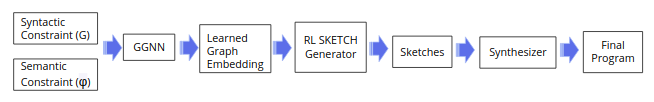
\includegraphics[width=\textwidth,height=2.0cm]{metasketcher.png}
\vspace*{-0.9cm}
\caption{META-SKETCHER Proposed Model}
\vspace{-1.2em}
\end{figure*}

\subsubsection{Formal Definitions}

Following are the formal definitions of some of the key terms.

\paragraph{Semantic Spec $\phi$ :}
These are formulas that consists of constraints written in the form of SMT formulae. It follows the same grammar G which is specified for the output program.

\paragraph{CFG G :}
A context free grammar (CFG) G is as defined in the [META-SOLVER] paper except the following modification.

The grammar should be modified for sketch generation by adding a new token <HOLE> which is used to replace any sub-tree in the program tree leaving that part to be searched using a symbolic search.

\paragraph{Output Sketch $\sigma$ :}
The Output Sketch $\sigma$ is a partial program generated using the grammar G. A good sketch will be the sketch that leads to final program f which satisfies both syntactic and semantic specifications.

\paragraph{Output Program f :}
The Output Program f is the final program that is generated from intermediate sketches. The final program f must satisy both syntactic (grammar G) and semantic (SMT formula $\phi$) specification 

\subsubsection{Novel Idea :}
Synthesizing sketches for General SyGuS benchmarks where the specifications are in the form of logical formulae instead of input output examples using a Reinforcement Learning framework. The policy network should learn to output partial programs based on the rewards.

\paragraph{Rewards :}
As sketches are incomplete programs it should not be verified by SAT/SMT solvers with the given semantic specification, one needs to consider some indirect ways of receiving rewards. Using the learned production probabilities, likelihood of the sketches could be calculated, and this can easily serve the purpose.


Both of these selected works does not talk about synthesizing programs for General SyGuS benchmarks. Also none has used sketches for it. As use of sketches in [SKETCHADAPT] has proved its applicability, I vouch for 

\subsection{Experiments}
\label{others}

\paragraph{Experimental Setup :}
Following experiments are done on Intel(R) Xeon(R) CPU E5-2420 v2 @ 2.20GHz with 32 GB Memory

\subsubsection{META-SOLVER}
I tested the META-SOLVER on 30 out of 214 SyGuS Cryptographic circuit synthesis benchmark problems. It elegantly solved 22/30 problems in an average time of $\sim0.32$ secs. While a state-of-the-art cvc4 ran out of memory for all the selected 30 problems. 

Because of less time, I could not perform a full fledged experiment as it requires more than 6 hours to conclude that a problem cannot be solved.\footnote{The SyGuS 2017 competition gives each solver 4-core 2.4GHz Intel processors with 128 GB memory and
wallclock time limit of 1 hour}

The excel sheet for the results can be found at \href{https://indianinstituteofscience-my.sharepoint.com/:x:/g/personal/raviraja_iisc_ac_in/EU-Um2g9igVJk5XrmXZoL1IBR_DlPHCtAWpxcVPZtu4n_Q?e=Krd9t5}{Excel Sheet for the Experments performed}

\subsubsection{Preliminary Results}
I did try to generate sketches using the existing framework of META-SOLVER but found that it is not able to handle infinite grammar (recursive grammar) and gives Recursion Error.

\subsection{Conclusion}
In this work I did a Literature Review for the field of Program Synthesis and it's improvements using Machine Learning. I exclusively reviewed the two recent tools for synthesizing programs one with sketches and other without sketches namely SKETCHADAPT and META-SOLVER respectively. The study shows that no work has been done around generating sketches for SyGuS problems where the specification is in the form of SMT formulae. The META-SKETCHER model presented in this work will be implemented in the near future.

\subsection*{References}
\small

[1] C. Cordell Green. Application of theorem proving to problem solving. In IJCAI, pages 219–240, 1969.

[2] Zohar Manna and Richard J. Waldinger. Toward automatic program
synthesis. Commun. ACM, 14(3):151–165, 1971.

[3] Richard J. Waldinger and Richard C. T. Lee. PROW: A step toward
automatic program writing. In IJCAI, pages 241–252, 1969.

[4] Rajeev Alur, Rastislav Bodík, Garvit Juniwal, Milo M. K. Martin,
Mukund Raghothaman, Sanjit A. Seshia, Rishabh Singh, Armando
Solar-Lezama, Emina Torlak, and Abhishek Udupa. Syntax-guided
synthesis. In Formal Methods in Computer-Aided Design, FMCAD,
pages 1–8, 2013.

[5] Oleksandr Polozov and Sumit Gulwani. FlashMeta: a framework for
inductive program synthesis. In Proceedings of the 2015 ACM SIGPLAN
International Conference on Object-Oriented Programming, Systems,
Languages, and Applications, OOPSLA 2015, pages 107–126, 2015.

[6] Sumit Gulwani. Automating string processing in spreadsheets using input-output examples. In Proceedings of the 38th ACM SIGPLANSIGACT Symposium on Principles of Programming Languages, POPL
2011, Austin, TX, USA, January 26-28, 2011, pages 317–330, 2011.

[7] Armando Solar-Lezama. Program synthesis by sketching. ProQuest,
2008.

[8] Aditya Krishna Menon, Omer Tamuz, Sumit Gulwani, Butler W. Lampson, and Adam Kalai. A machine learning framework for programming by example. In Proceedings of the 30th International Conference on Machine Learning, ICML 2013, Atlanta, GA, USA, 16-21 June 2013,
pages 187–195, 2013.

[9] Devlin, J., Uesato, J., Bhupatiraju, S., Singh, R., Mohamed,
A.-r., and Kohli, P. Robustfill: Neural program learning
under noisy i/o. arXiv preprint arXiv:1703.07469, 2017.

[10] Matej Balog, Alexander L. Gaunt, Marc Brockschmidt, Sebastian
Nowozin, and Daniel Tarlow. DeepCoder: Learning to write programs.
CoRR, abs/1611.01989, 2016.

[11] Maxwell I. Nye, Luke B. Hewitt, Joshua B. Tenenbaum, and Armando Solar-Lezama. Learning to
infer program sketches. In Kamalika Chaudhuri and Ruslan Salakhutdinov (eds.), Proceedings
of the 36th International Conference on Machine Learning, ICML 2019, 9-15 June 2019, Long
Beach, California, USA, volume 97 of Proceedings of Machine Learning Research, pp. 4861–4870.
PMLR, 2019.

[12] X. Si, Y. Yang, H. Dai, M. Naik, and L. Song, “Learning A Metasolver For Syntax-guided Program Synthesis,” ICLR, 2018.

[13] Hassan Eldib, Meng Wu, and Chao Wang. Synthesis of fault-attack countermeasures for cryptographic circuits. In Swarat Chaudhuri and Azadeh Farzan (eds.), Computer Aided Verification, 2016.

%Ravi
